The contents of this chapter are motivated by common practical use-cases in which machine learning is applied. Often, data are collected as a combination of multiple conditions, e.g. the voice recordings or medical images of multiple persons, each labeled with an identifier for each person. How could we build a model that captures the latent information related to these conditions and generalizes to a new one with few data? 

\section{Motivation: Meta-Learning}
Deep learning models, unfortunately, usually need millions of labeled samples to be trained. However, in some applications such as medical image analysis, this requirement cannot be fulfilled since (labeled) samples are hard to collect. On the other hand, a remarkable aspect of human intelligence is the ability to quickly solve a new problem and to be able to do so even with limited experience. Such fast adaptation is made possible by leveraging prior learning experience in order to improve the efficiency of later learning. That is, humans while learning tasks are also able to learn \say{how to learn}. This capability for \say{meta-learning} also has the potential to enable an artificially intelligent agent to learn more efficiently in situations with little available data or limited computational resources.

In machine learning, meta-learning is formulated as \say{[...] the extraction of domain-general information that can act as an inductive bias to improve learning efficiency in novel tasks} [\cite{Grant2018}]. 

Meta-learning attempts to endow machine learning models with the ability to learn from small data leveraging past experience by training a meta-learner to perform well on a \textit{distribution} of training tasks. The meta-learner is then applied to an unseen task, usually assumed to be drawn from a task distribution similar to the one used for training, with the hope that it can learn to solve the new task efficiently. Therefore, for problems in which data are insufficient, meta-learning is a good solution if there are multiple related tasks. 

In meta-Learning (or Learning-to-Learn or Inductive Transfer) a \textit{meta-learner} extracts knowledge from several observed tasks to facilitate the learning of new tasks by a \textit{base-learner}, see fig. (\ref{fig:meta_learning}). 
%In this setup the meta-learner must generalize from a finite set of observed tasks. 
The performance is evaluated when learning related new tasks (which are unavailable to the meta-learner). In other words, meta-learning is a way to \textit{learn a prior}. 
%Therefore, the goal of meta-learning is to train a model on a variety of learning tasks, such that it can solve new learning tasks using only a small number of training samples. 
\begin{figure}
    \centering
    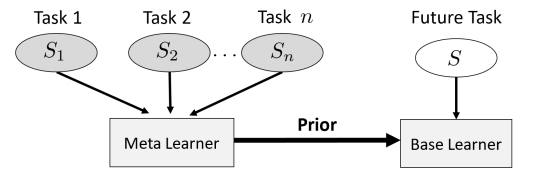
\includegraphics[scale=0.5]{images/meta.png}
    \caption{The meta-learner uses the data sets of the observed tasks $S_1, \dots, S_m$ to infer \textit{prior knowledge} which in turn can facilitate learning in future tasks from the task-environment.}\label{fig:meta_learning}
\end{figure}

To summarize, meta-learning allows an intelligent agent to leverage prior learning episodes as a basis for quickly improving performance on a novel task. Bayesian hierarchical modeling provides a theoretical framework for formalizing meta-learning as inference for a set of parameters that are shared across tasks.

%Formally, we consider a \say{population} of tasks, but we only get to observe only a sample of size $K$ of all possible tasks, $\mathcal{T}_1,\dots, \mathcal{T}_K$ hence we define a distribution over tasks, $p(\mathcal{T})$. These tasks share some common structure such that learning to solve a single task has the potential to provide information to solve another. Each task, $\mathcal{T}_k$, defines a distribution over data points $D_k$, which we assume in this work to consist of inputs and targets, that is $D_k = \{x_{i,k}, y_{i,k}\}_{i=1}^{N_k}$, where $N_k$ is the number of observed data in task $k$. The objective of the meta-learner is to be able to minimize a task-specific performance metric associated with any given unseen task from the dataset given even only a small amount of data from the task.

%The learning tasks differ in the unknown sample distribution $p(D_k)$ associated with each task. The meta-learning agent observes the training sets $D_1,\dots,D_K$ corresponding to $K$ different tasks. Each observed dataset $D_k$ is assumed to be generated from an unknown sample distribution $(x^{(m)}, y^{(m)}) \sim G_m$. The sample distributions $G_m$ are generated i.i.d. from an unknown tasks' distribution $G_0$. The goal of the meta-learner is to extract some knowledge from the observed tasks that will be used as prior knowledge for learning new (yet unobserved) tasks from $G_0$. The prior knowledge comes in the form of a distribution over the parameters of the distribution of the tasks. When learning a new task $T_{k+1}$, the base learner uses the observed task’s data $D_{k+1}$ and the learned \say{prior}, $G_0 | D_1,\dots,D_m$, to output a posterior distribution $G_{m+1}|D_{m+1}$. We assume that all tasks are learned via the same learning process. 

\bigbreak 

We introduce the next section with a practical example which highlight the common use-case of meta-learning. We often collect data as a combination of multiple \say{scenarios} or \say{tasks}, in the machine learning parlance. This different scenarios can be, for example, images taken from different models of cameras. We only have some labels to identify these scenarios in our data, e.g. we can have the specifications of the used cameras. These labels themselves do not represent the full information about these scenarios. Therefore, we could wonder \textit{how to use} these labels in a supervised learning task. A common practice in this case would be to ignore the difference of scenarios, but this will result in low accuracy of modeling, because all the variations related to the different scenarios are considered as observation noise, as different scenarios are not distinguishable anymore in the inputs. Alternatively, we can either model each scenario separately, which often suffers from too small training data, especially if we want to train a deep model. In both of these cases, generalization to new scenario (or task) is not possible.

In this chapter, we address this problem by reviewing a probabilistic model that can jointly consider different scenarios and enables efficient generalization to new scenarios. This model is based on Gaussian Processes (GP) augmented with additional latent variables and deep neural nets. The model is able to represent the data variance related to different scenarios in the latent space. This allows the model to efficiently and robustly generalize to a new scenario. An efficient Bayesian inference scheme, developed by deriving an amortized variational lower bound and a particular training regime make it more scalable than GPs.


\section{Neural Processes}
Neural Processes have been introduced recently by the two seminal papers [\cite{Garnelo2018a, Garnelo2018b}]. Differently from these papers, we will introduce them in the context of Bayesian nonparametric regression, therefore insisting on their probabilistic interpretation. In doing so, we will start with a motivating example inspired by [\cite{Dai2017a}].


\subsection{Motivating Example}
Consider a situation in which we wish to model the braking distance of a car in a completely data-driven way, that is, assuming no knowledge about physics. We can treat it as a nonparametric regression problem, where the input is the initial speed and the output is the distance from the location where the car starts to brake to the point where the car is fully stopped. We know that the braking distance depends on the friction coefficient, which varies according to the conditions of tyres and road. 

To measure the friction coefficient we can conduct experiments with a set of different tyres and road conditions, each associated with a condition identifier. We can think of something like ten different conditions, each has five experiments with different initial speeds. How can we model the relation between the speed and braking distance in a data-driven way, so that we can extrapolate to a new condition with only one experiment?

\bigbreak

To formalize the problem we denote the speed to be $x$ and the observed braking distance to be $y$ and the condition identifier to be $\tau$ -- for \say{task}. As said in the introductory section, one modeling choice is to ignore the difference in conditions. Since we do not know the parametric form of the function, we model it nonparametrically. Then, the relation between the speed and distance can be modeled simply as
\begin{equation*}
    y = f(x) + \varepsilon, \qquad f\sim p(f)
\end{equation*}
where $\varepsilon$ represents measurement noise and the function $f$ can be modeled, for example, as a Gaussian Process. As noted above, the drawback of this model is that the variations caused by different conditions are modeled as measurement noise and thus accuracy results very low.

Alternatively, we can model each condition separately, that is, 
\begin{equation*}
    y = f_\tau(x) + \varepsilon, \qquad f_\tau\sim p(f), \quad \tau = 1,\dots,\mathcal{T}
\end{equation*}
where $\mathcal{T}$ denotes the number of considered conditions. In this case, the relation between speed and distance for each condition can be modeled only if there are sufficient data in that condition. Even if this is possible, the model is not able to generalize to new conditions because it does not consider the correlations among conditions.  

Our goal is to model the relation between inputs and outputs together with the latent information associated with different conditions. A probabilistic approach, which underlies the construction of neural processes as well, is to assume a latent variable, $z$, that represents the latent information associated with the condition (or task) $\tau$. The input-output relation is, then, modeled as 
\begin{equation}\label{eq:regz}
    y = f(x, z) + \varepsilon, \qquad f \sim p(f), \quad z \sim p(z)
\end{equation}
Note that the function $f$ is shared across all conditions while for each condition a different latent variable $z$ is inferred. The problem is cast as a Bayesian random effect regression problem. In this way all the conditions are modeled jointly letting the correlation among different conditions to be correctly captured. This allows for generalization to new conditions (or tasks). 

To summarize, neural processes find suitable application in supervised problems involving \textit{multiple responses} that we would like to model as \textit{conditionally dependent}. In statistical terminology, this entails \textit{sharing} or \textit{borrowing} \textit{statistical strength} between multiple response variables that, as noted in the introduction to the chapter, in machine the learning parlance is referred to as meta-learning.  



\subsection{Stochastic Process Approximators}
A possible way to model the \textit{multiple responses} problem -- as we have labeled it at the end of the previous section -- is to assume that underlying the relation between inputs and outputs there is a stochastic process.

A stochastic (or random) process is described by some function $f(x)$ where $x$ assumes values in a reference set $\mathcal{X}$. As $x$ varies, $f(x)$ describes the evolution of the process. The way in which the process evolves is random, and each of the functions $f(\cdot)$ describes only \textit{one} of the possible ways in which the process may develop. This functions $f(\cdot)$ are called \textit{sample functions} of the stochastic process [\cite{GikhmanSkorokhod1969}]. In other words, for each fixed $x$, the quantity $f(x)$ is random. It is natural to assume that $f(x)$ is a random variable in the probabilistic sense. Consequently, by a stochastic process we mean a family of random variables $f(x)$ indexed by $x$ that assume values in some set $\mathcal{X}$. Therefore, a stochastic process defines a distribution over functions, this motivates the alternative name \textit{random function}.

In our interpretation, each condition or task or response or dataset -- as we may wish to refer to them -- can be considered as \textit{one} realization of the underlying stochastic process, i.e. a single instantiation of the random function. The distribution over datasets, therefore, allows us to learn the distribution of the random functions. 

A Neural Process, therefore, describes a stochastic process. It learns to approximate a stochastic process exploiting the information derived from multiple datasets, or single instantiation of the random function -- as we have labelled them. 

Considering again our regression problem, eq. \eqref{eq:regz}, we motivated the introduction of $z$ as a latent factor identifying the different conditions (or tasks). We refer to this modeling approach as bottom-up construction. We can derive an equivalent model adopting a top-down approach. 

We assume that the different datasets are realizations of the true underlying stochastic process. A possible way to describe a random function is using a latent random variable $z$ to parameterize a \textit{deterministic} function $f_z$. In this way we can model different realizations of the data generating stochastic process: each sample of $z$ corresponds to one realization of the stochastic process. It this sense $z$ is a \textit{global} latent variable: once sampled, an entire function is defined, not just one data point. In other words, given $x$, $f_z(x)$ is random since $z$ is random: the randomness in $f$ is conveniently moved to $z$.

To formalize the problem, consider the inputs $x\in\mathcal{X}$ and the outputs $y\in\mathcal{Y}$. Define $\mathcal{M}(\mathcal{Y})$ the space of all probability measures (distributions) over $\mathcal{Y}$. Then $f_z: \mathcal{X}\to\mathcal{M}(\mathcal{Y})$ is a random function, whose randomness depends one the randomness of $z$, which maps each input $x\in\mathcal{X}$ into a distribution over the corresponding output $y\in\mathcal{Y}$.  

To sum up, a Neural Process is one specific way to define the functions $f_z$ and, thus, we refer to it as \textit{stochastic process approximator}. 



\subsection{The Model: Definition and Objective}
Consider the regression problem of eq. \eqref{eq:regz}
\begin{equation*}
    y = f(x, z) + \varepsilon, \qquad f \sim p(f), \quad z \sim p(z)
\end{equation*}
Where $f$ is shared across all tasks. In section (\cref{sec:BNPreg}) we refered to this kind of models as \textit{nonparametric mean function regression}. Let $\mathcal{F}$ be some class of regression functions on which the probability measure $p(\mathcal{F})$ is defined. The peculiarity of NPs is that $\mathcal{F}$ is defined to be the class of neural networks. We define a generic element of this class as $g_\theta$, indexed by a parameter vector $\theta\in\Theta$. This modeling approach liberates the practitioner from having to specify a prior for $f$, e.g. a Gaussian Process, since it will be inferred from the data.

The error term is assumed to be normally distributed with mean zero and diagonal covariance matrix: this guarantees that $g_\theta$ can be interpreted as the conditional mean function. Furthermore, in line with the literature about variational autoencoders, section (\cref{sec:vae}), $p(z)$ is assumed to be a multivariate Gaussian. To define a Neural Process we can rewrite eq. \eqref{eq:regz} according to these assumptions 
\begin{equation*}
    y = g_\theta(x,z) + \varepsilon, \qquad \text{$z\sim \mathcal{N}\left(\mu_z,\sigma_z^2 I\right)$ and $\varepsilon\sim\mathcal{N}\left(0,\sigma^2 I\right)$}
\end{equation*}
where $\varepsilon$ is measurement noise and $\theta$ represents learnable parameters of the neural net. Since, given a specific $z$, $g_\theta$ is deterministic and the covariance matrix is diagonal, the outputs $y_i$'s are \textit{i.i.d.} Gaussian random variables. Given $N$ input-output pairs (across all tasks) we can write the generative model as
\begin{align*}
    p(y,z|x) &= p(z) \; p(y|z, x)\\
             &= \mathcal{N}\left(\mu_0,\Sigma_0\right) \; \prod_{i=1}^{N}\mathcal{N}\left(g_\theta(z, x_i), \sigma^2\right)
\end{align*}
Bayesian inference for this model implies the computation of the posterior distribution $p(z|y,x)$. 

To approximate this posterior, as for VAE (sec. \cref{sec:vae}), we can use amortized variational inference. We define the variational distribution to be 
\begin{equation*}
    q_\phi(z|x) = \mathcal{N}\left(\mu_z(x), \sigma^2_z(x)I\right)
\end{equation*}
as for conditional variational autoencoders, where the conditioning on $x$ indicates that the variational parameters are replaced by functions of the data. Specifically, these functions, $\mu_z(\cdot)$ and $\sigma^2_z(\cdot)$ are neural networks with a peculiar structure that makes them invariant to the order of the inputs, and $\phi$ represents the parameters of the networks. 

To obtain an estimate of the posterior, we minimize $\mathrm{KL}[q_\phi(z|x)\Vert p(z|y,x)]$. Since this involves the computation of intractable distributions, as in section (\cref{sec:generic VI}), we minimize another tractable objective: the ELBO, that following the same rationale explained in that section, can be written as
\begin{equation}\label{eq:NPelbo}
    \mathrm{ELBO}(\phi) = \mathrm{E}[\log p(y|z,x)] - \mathrm{KL}[q_\phi(z|x)\Vert p(z)]
\end{equation}
where we know that $\log p(y|x) \geq \mathrm{ELBO}(\phi)$ from section (\cref{sec:VI}). Thus, maximizing the ELBO is approximately equal to maximizing the joint distribution of the outputs given the inputs.



\subsection{A Peculiar Training Regime}
NPs are designed to learn distributions over functions from distributions over datasets. Consider a set of datasets (or tasks), $\mathcal{D}$. For each dataset, $\mathcal{D}_\tau \in \mathcal{D}$ we have $N_\tau$ input-output pairs $\{(x_i^{(\tau)}, y_i^{(\tau)})\}_{i=1}^{N_\tau}$, where $N_\tau$ is the size of dataset $\tau$, for $\tau\in\{1,\dots,\mathcal{T}\}$. The total number of training data is $N = N_1 + \dots + N_\mathcal{T}$.

At each iteration of learning, one dataset $\mathcal{D}_\tau = \{(x_i^{(\tau)},y_i^{(\tau)})\}_{i=1}^{N_\tau}$ is chosen. A subset, referred to as \textit{context set}, $C_\tau = \{(x_i^{(\tau)},y_i^{(\tau)})\}_{i=1}^{M_\tau}$ is randomly sampled. Symmetrically, the entire dataset is called \textit{target set}, that is, $T_\tau = \mathcal{D}_\tau$. Usually $M_\tau\leq N_\tau$ and is also randomly chosen, that is, $M_\tau \sim \mathrm{Unif}(0, N_\tau)$. For brevity, once a dataset is chosen amongst all datasets, let $x_C, y_C, x_T, y_T$ denote the inputs and outputs of the context and target set respectively.

The NP during training can learn from the context points only and must predict the target points, i.e. the the entire dataset (or function, or realization of the stochastic process). The ELBO in eq. \eqref{eq:NPelbo} does not reflect this division into context and target set. In fact, we are requiring the NP to maximize the joint distribution of all outputs (the target set, as we have defined it) given no context -- which is the standard variational lower bound. We label this kind of objective function as $\mathrm{ELBO}_{[T|\varnothing]}$.

To better reflect the training regime of the NPs, instead of maximizing the joint distribution of all outputs, i.e. the target set, given no context, we can maximize the conditional distribution of the target given the context. This lead to the objective
\begin{equation}\label{eq:ELBOcond}
    \mathrm{ELBO}_{[T|C]}(\phi) = \mathrm{E}[\log p(y_T|z,y_C, x_C)] - \mathrm{KL}[q_\phi(z|y_C, x_C)\Vert p(z|y_C, x_C)]
\end{equation}
where we know that $\log p(y_T|x_T, x_C, y_C) \geq \mathrm{ELBO}_{[T|C]}$. Note that $p(z|y_C, x_C)$ is a \textit{conditional prior} [\cite{Garnelo2018b}], that can be interpreted as a less informed posterior.



\subsection{Stochastic Approximation of the ELBO}
Since the ELBO contains (possibly deep) neural networks, an analytic evaluation of it is hard to obtain. In such cases, as we have seen in section (\cref{sec:generic VI}), it is possible to use black-box variational inference. In particular, we use the reparametrization trick to obtain an estimate of the ELBO by Monte Carlo samples.

We reparametrize $z$ as a transformation of a random variable $\eta \sim \mathcal{N}\left(0, I\right)$, that is
\begin{equation*}
    z = \mu_z(x) + \sigma_z(x) \eta 
\end{equation*}
The expectations involved in the ELBO are, thus, computed with respect to the distribution of $\eta$. As for the conditional variational autoencoder, for each data point, we sample $S$ times $\eta_{i,s}$ from a noise distribution $p(\eta) = \mathcal{N}(0,I)$. Once we have $S$ instantiation of the latent variable corresponding to one dataset, $z_s =  \mu_z(x) + \sigma_z(x) \eta_{i,s} $, for each data point, we can approximate the per-data point ELBO using the following Monte Carlo estimate
\begin{equation*}
    \widehat{\mathrm{ELBO}}_{[T|C]}(x_i, \phi, \theta) \approx \frac{1}{S}\sum_{s=1}^{S} \log p(y_i|x_i, z_{s}) - \mathrm{KL}[q_\phi(z|x_i, y_i)\Vert p(z|x_i)]
\end{equation*}
As shown in section (\cref{sec:reparametrization}), the gradient of the ELBO can be easily computed, given the new parametrization. However, note that in this case we do not have the subscript $i$ in $z$. This is motivated by the fact that $z$ in NP represents global uncertainty, that is, it is sampled once for all points in a dataset (or task), it is not sampled for each single data point.



\subsection{Encoder Specification}
As we defined it in section \cref{sec:vae}, the approximating distribution $q_\phi$ is also called \textit{encoder}. The authors, in building the NP [\cite{Garnelo2018a, Garnelo2018b}], designed the encoder in such a way to accommodate \textit{invariance to the order} of context points. Therefore, the neural nets $\mu_z$ and $\sigma^2_z$ have both a peculiar structure. 

The architecture used can be boiled down to three core components
\begin{itemize}
    \item A neural net $h$, that the authors refer to as \textbf{encoder} -- even if the encoder is usually used to refer to the entire approximating distribution -- that maps the input space into the representation space; it takes pairs $(x_i, y_i)_{i\in C}$ in the context set and produces a representation $r_i = h(x_i, y_i)$ for $i\in C$
    \item An \textbf{aggregator} $a$, that summarizes the encoded inputs in an order-invariant global representation $r = a(r_i)_{i\in C}$; they implement the aggregator as a mean function, perhaps the simplest operation that ensures order-invariance
    \item Two neural nets $\mu$ and $\sigma^2$ that map the global representation to the mean and variance of the global latent variable; in practice they have the same architecture, but a transformation that ensures positive outcomes is added at the end of the $\sigma^2$ network 
\end{itemize}
Therefore, $\mu_z \stackrel{\scriptscriptstyle def}{=} \mu(a(h(x_i, y_i)))$ and $\sigma^2_z \stackrel{\scriptscriptstyle def}{=} \sigma^2(a(h(x_i, y_i)))$, for $i\in C$.

\bigbreak 

To summarize, NPs have three main desirable properties [\cite{Garnelo2018a}]: 
\begin{itemize}
    \item \textit{Scalability}: since they rely on amortization
    \item \textit{Flexibility}: since they define a wide family of distributions and one can condition on an arbitrary number of context points to obtain an arbitraty number of targets
    \item \textit{Permutation invariance}: given by the construction of the encoder
\end{itemize}
Therefore, like Gaussian Processes, NPs define distributions over functions, are capable of adaptation to new observations, and can estimate uncertainties in their predictions. Like neural networks, they are computationally efficient during both training and evaluation, and in addition learn to adapt their priors to the data.


